%\chapter{Conclusão} - manter comentado

	\begin{flushright}
		\textit{``Palavras não bastam, não dá pra entender\\
                    E esse medo que cresce não para\\
                    É uma história que se complicou\\
                    Eu sei bem o porquê ''\\Tiê}
	    \end{flushright}
	    
	    Logo ao comparar estes geradores percebemos que a biblioteca nativa do java trás benefícios ao ser mais facilmente incluído em um código por ser nativo, mas possui o contra onde para que seu período não seja somente entre 0 e 1, e para burlar isso os seus valores precisam passar por operações matemáticas aplicadas por aquele que esta escrevendo o código.
	    
	    Já o gerador implementado nos testes anteriores possui também seus prós e contras, este exige sua implementação e até mesmos ajustes de acordo com onde será utilizado e também necessite de um estudo de um modulo, um multiplicador, e um incremento para construir um período que atenda as necessidades, mas este possui o beneficio de sua simplicidade e uma execução sem muito custo computacional.
	    
	    Também foi possível comparar o tempo de execução entre estes algoritmos, e perceber que o PRNG implementado manualmente supera em a biblioteca do java no quesito velocidade para preencher um vetor com valores gerados por estes métodos, veja um exemplo de resultado na imagem a seguir:
	    
	    \begin{figure}[ht]
            \centering
            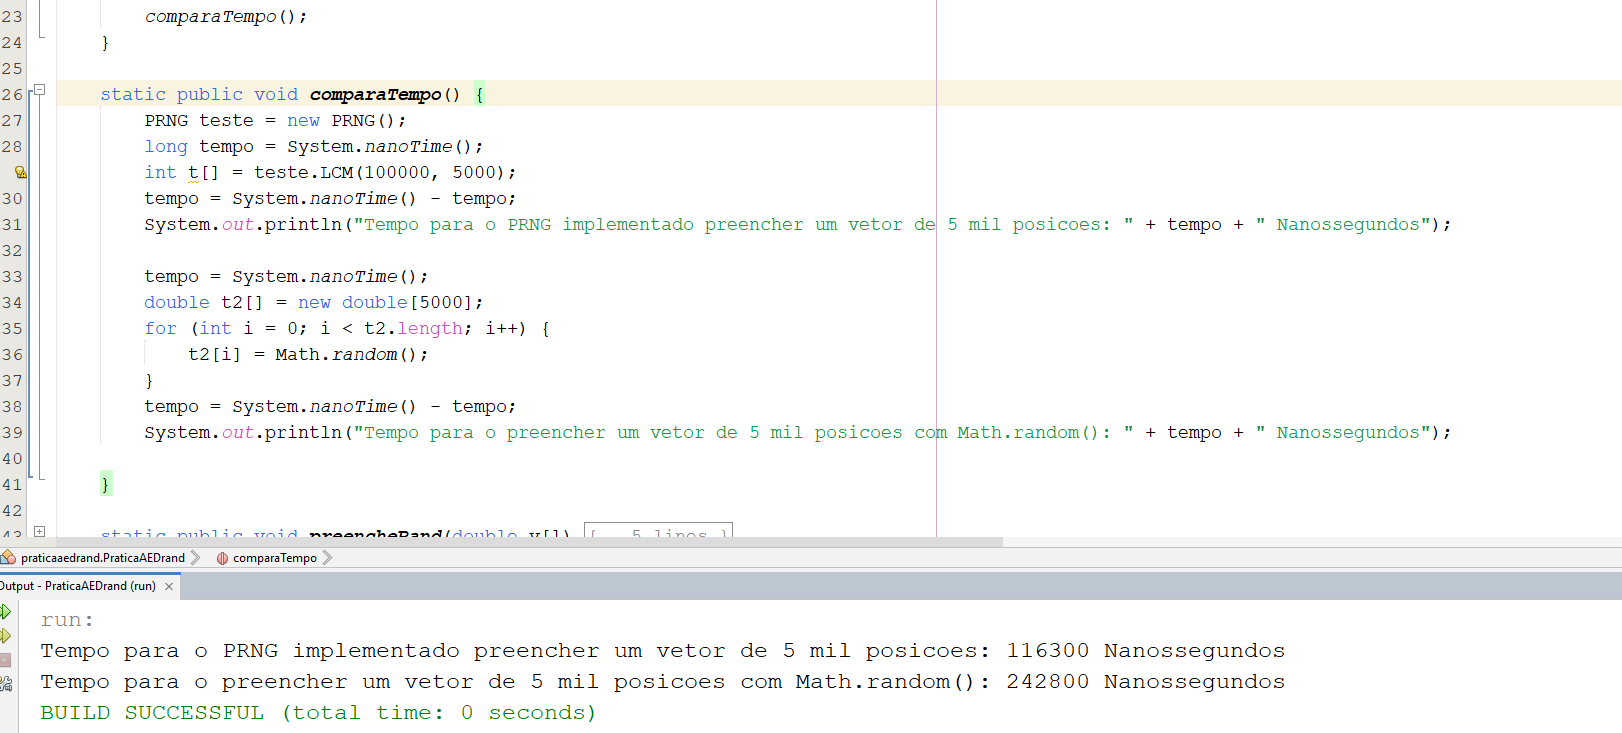
\includegraphics[scale=0.4]{JoseGeraldo-lista2/fig/fig6.png}
            \caption{Comparação de tempos de execução}
        \end{figure}
        
    \pagebreak
	    Por fim o mais importante a se concluir com este experimento é que não podemos considerar estes geradores como aleatórios, estes possuem sim um padrão de resultados que pode ser ilustrado.
	    Mas o importante é que mesmo sendo pseudo aleatórios estes não deixam de ser uteis e em determinadas implementações cumprem o papel de geradores aleatórios.